In this chapter, we go over the implementation details of the BlockLearning framework, following the guidelines defined in \Cref{chapter:methodology}. The complete implementation is publicly available on GitHub\footnote{\url{https://github.com/hacdias/blocklearning}}.

\section{Smart Contracts}

The first part of the framework is the smart contracts. As mentioned previously, this work uses the Ethereum\footnote{\url{https://ethereum.org/en/}} blockchain platform. Therefore, the smart contracts must be implemented in a programming language that supports Ethereum. We chose the Solidity\footnote{\url{https://soliditylang.org/}} programming language as it is the most well-known with the widest support.

Since our framework supports different techniques with different requirements, we implemented four different smart contracts. These smart contracts inherit most of their functionality from an abstract smart contract that provides the common data structures and functionality, named \texttt{Base}. Then, we implement the following classes, that derive from \texttt{Base}:

\begin{itemize}
    \item \texttt{NoScoring}, which is used when we do not need a scoring mechanism. It only adds a new function to the \texttt{Base} class in order to allow the owner to start a round.
    
    \item \texttt{Scoring}, which is used when we need a scoring mechanism. This smart contract implements the required methods to support the scoring phase, such as scoring submissions and the scoring round.
    
    \item \texttt{FirstComeFirstServed}, which is used with the "first come, first served" participant selection technique. It overrides some of the \texttt{Base} functions in order to register participants to the round as they submit their updates.
    
    \item \texttt{Vertical}, which is used with vertically partitioned data, specifically with the Split-CNN. It incorporates the functionality required to provide for an additional phase, the backpropagation, as well as more information about the head and top models.
\end{itemize}

A class diagram with the public interfaces of the contracts, as well as the data types, is depicted \autoref{fig:contracts-uml}. An interesting aspect to note is that score and accuracy values are stored as integers. Currently, Solidity does not support floating point numbers. To preserve fidelity, the original values are multiplied by a large integer, $10^{18}$. Then, when the values are retrieved from the smart contract, they are divided by the same value in order to get the original value.

\begin{figure}[!ht]
    \centering
    \centering
    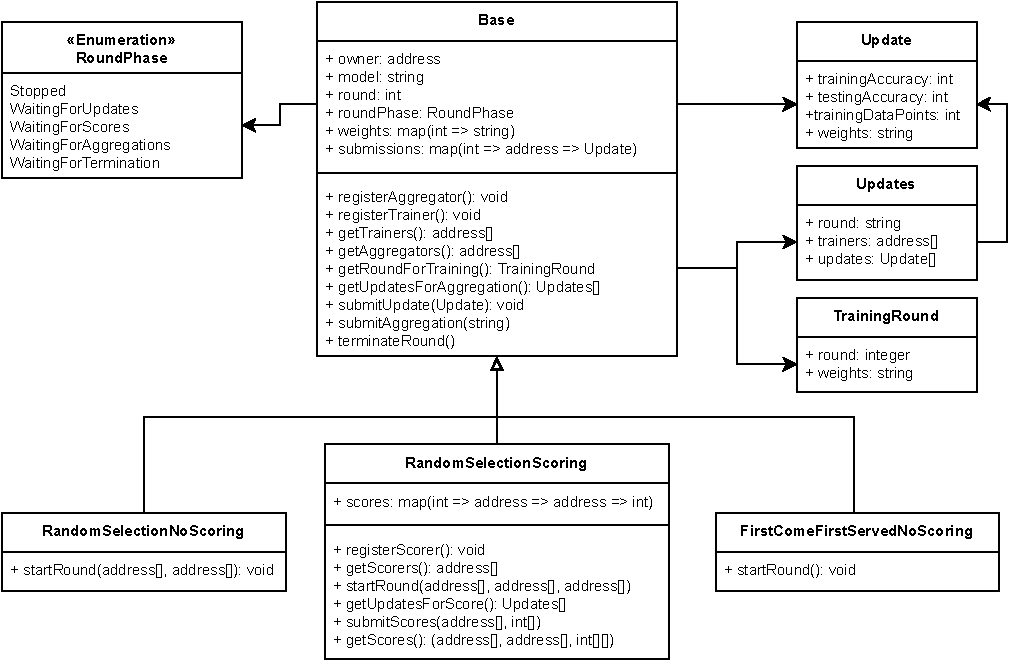
\includegraphics[width=1\textwidth]{graphics/smart-contract-uml.pdf}
    \caption{Smart Contracts Class Diagram}
    \label{fig:contracts-uml}
\end{figure}

\section{Library}

The library is implemented in the Python\footnote{\url{https://www.python.org/}} programming language. The main motivation for using Python is that many well-known Machine Learning libraries, such as TensorFlow\footnote{\url{https://www.tensorflow.org/}} and PyTorch\footnote{\url{https://pytorch.org/}} are implemented in Python, as well as many data processing tools.

The first part of the library is the aggregation, scoring and privacy algorithms. Each of these categories of algorithms has a specific interface to which each algorithm must conform to. By having a common interface, we can implement new algorithms, or change existing ones, easily. The interfaces are as follows:

\begin{itemize}
    \item \texttt{aggregate(trainers, updates, scorers, scores) $\rightarrow$ weights}\\
    The aggregators must provide a function \texttt{aggregate} that receives an array with the trainer addresses, an array with the updates sorted by the same order as the trainers, an array with the scorers and an array with the scores sorted by the same order as the scorers. It is important to note that the scorers and the scores are optional arguments since a scoring algorithm is not always required. The function returns an array with the aggregated weights. % BlockFlow, FedAvg, Multi-KRUM
    
    \item \texttt{score(round, trainers, updates) $\rightarrow$ trainers, scores}\\
    The scorers must provide a function \texttt{score} that receives an integer with the round number, an array with the trainer addresses, as well as an array of updates that are sorted by the same order as the trainer addresses. The function returns an array with the trainers and their submission scores. % Multi-KRUM, MarginalGain, Accuracy (BlockFlow)
    
    \item \texttt{privatize(x) $\rightarrow$ y}\\
    The privacy mechanisms must provide a function \texttt{score} that receives an array of the weights \texttt{x} and returns the privatized weights \texttt{y}. % Gaussian
\end{itemize}

The second part of the library is the utilities to store and retrieve the weights, as well as the smart contract bridge. The weights storage class also provides a common interface such that it is possible to change which storage provider we use. As for our experiments, we use IPFS, explained in \Cref{background:ipfs}, similarly to many other works. The smart contract bridge is a class that creates a 1:1 connection with the functions from the smart contracts.

The third and final part of the library is the \texttt{Trainer}, \texttt{Scorer} and \texttt{Aggregator} classes. These classes implement the main flow of each of these procedures using the modules aforementioned described. For example, the trainer class is initialized with the contract bridge, the weights storage, the model, the data and an optional privacy mechanism. Then, it provides a method \texttt{train()} that executes the training procedure. Similarly, the scorer class provides \texttt{score()} and the aggregator class provides \texttt{aggregator}.

\section{Testbed}

The testbed, that is, the platform to conduct the experiments. It was mostly implemented using the aforementioned library and Docker\footnote{\url{https://www.docker.com/}}. Docker is a platform that allows to easily deploy applications in an isolated setting through what is called a container, allowing us to simulate multiple devices in the same network. Each container runs an image, which is the name given to the piece of software than runs on the container.

In the testbed, we have two major components: the client, server and owner scripts, the federated learning environment deployment and the blockchain deployment. These are discussed on the following subsections.

\subsection{Client, Server and Owner Scripts}

The client, server and owner scripts are the processes that will run at the client, server and owner, respectively. These are implemented using the BlockLearning library. In each of these processes, we first load the required data, such as the data set in the clients, and initialize the required mechanisms, namely the scoring, aggregation and privacy mechanisms.

Then, depending on the scoring mechanism, we initialize the relevant classes at the correct machines. For example, for the BlockFlow scoring algorithm, the client initializes a \texttt{Trainer} and a \texttt{Scorer}, while the server initializes an \texttt{Aggregator}. In contrast, for Multi-KRUM, the client only initializes a \texttt{Trainer}, while the server initializes an \texttt{Aggregator} and a \texttt{Scorer}. On \autoref{alg:client_loop} you can visualize part of the main loop of the  client script.

\begin{algorithm}
\caption{Client Script Main Loop}\label{alg:client_loop}
\begin{algorithmic}
\Require $s \in$ \{\O, BlockFlow, MarginalGain\}
\State $T \gets $ Initialize Trainer
\If{$s$ is not \O}
    \State $S \gets $ Initialize Scorer
\EndIf
\While{True}
    \State $P \gets$ Get Phase From Smart Contract
    \If{$P$ is Waiting For Updates}
        \State Execute Training Procedure $T$
    \ElsIf{$P$ is Waiting For Scores}
        \State Execute Scoring Procedure $S$
    \EndIf
\EndWhile
\end{algorithmic}
\end{algorithm}

\subsection{Blockchain Setup and Deployment}

The Blockchain setup and deployment is done using already existing tools and our library. As previously mentioned, we use Docker containers in order to run the experiments. Moreover, we use Docker Compose in order to deploy multiple containers at once and orchestrate the deployment process.

We use different Ethereum implementations, depending on the consensus algorithm since they are not all available within the sample implementation. Ethereum's main implementation, \texttt{go-ethereum}\footnote{\url{https://github.com/ethereum/go-ethereum}}, provides PoA and PoW. For QBFT, we use a fork called \texttt{quorum}\footnote{\url{https://github.com/ConsenSys/quorum}}, which is mostly identical to \texttt{go-ethereum} but supports QBFT.

Moreover, the Blockchain setup and deployment follows the following steps:

\begin{enumerate}
    \item \textit{Generate Accounts}. In first place, the Ethereum accounts for the clients and servers are generated using the provided \texttt{go-ethereum} toolkit. Each account is pre-loaded with $100$ ETH, the Ethereum currency, so that clients or servers will not run out of currency to submit their transactions.
    
    \item \textit{Build Images}. In second place, we build the Docker images that will be used to deploy the Blockchain network. This images are based on the images provided by each of the Ethereum's implementations that we use. In addition, they pre-load the account information, as well as some additional configuration to ensure that all nodes are connected when the network is bootstrapped.
    
    \item \textit{Deploy Network}. In third place, the network is deployed using Docker Compose and the configured amount of nodes.
    
    \item \textit{Deploy Contract}. Finally, the contract is deployed to the network using Truffle, which is a tool designed to help developers developing and deploying smart contracts.
\end{enumerate}

Finally, we would like to mention that originally we were planning on testing the PoS consensus algorithm too. However, the only fork providing PoS support does not work in private network settings\footnote{\url{https://github.com/bnb-chain/bsc/issues/861}}. Therefore, it was not possible to run an experiment with PoS.

\subsection{Federated Learning Setup and Deployment}

Similarly to the Blockchain setup and deployment, we also use Docker Compose for the Federated Learning system. The process is identical as in the previous section, except that we only build the images and deploy the Federated Learning network.

\subsection{Statistics}

Statistics, necessary for the metrics described in \Cref{meth:metrics}, are collected using Docker's own tool \texttt{docker stats}. Docker statistics\footnote{\url{https://docs.docker.com/engine/reference/commandline/stats/}} provides a live stream of each container's resource consumption, namely the CPU percentage, the RAM memory usage, and the network traffic in and out.

Other statistics, such as accuracy and score values, are collected via log hooks embedded into the \texttt{Trainer}, \texttt{Scorer} and \texttt{Aggregator} scripts. This JSON logs are then post-processed to CSV, which we then use to create the necessary plots and tables to analyze the results.
